\chapter{高效的基于变分推断的高阶依存句法分析}\label{cha:approximate-vi}

本章节提出了一个采用消息传递机制的二阶基于图的和端到端神经网络模型.
这里我们从经验上表明,我们采用的近似方法不仅从准确率上可以与章节~\ref{cha:dep-crf}里提出的二阶基于图的解析器相匹敌,并且其训练和测试的速度都要远远快于二阶CRF解析器.

\section{引言}\label{sec:vi-intro}
基于图的依存句法分析一直以来都是依存句法分析领域的一个比较流行的方法.
在本章节中,我们在章节~\ref{cha:dep-crf}的基础上继续探索基于图的依存句法分析,即给定一个句子,选择将句子分解为多个部分并对他们打分,进而选择分值最高的句法树.

一阶基于图的依存句法分析将一棵完整的句法树分解为多条弧,将每条弧都视为一个独立的部分.
在深度学习时代之前,已经有大量的方法被提出用于一阶依存句法分析\cite{mcdonald-pereira-2006-online,koo-etal-2007-structured,ma-hovy-2017-neural,dozat-etal-2017-biaffine}.

这些方法通常依赖于大量的手工特征的设计,以及结构化学习方法,比如Max Margin、TreeCRF和Matrix Theorem等等,这些方法通常显示建模树的约束,更新参数使得模型尽可能预测出正确的树结构.
得益于深度神经网络的强大上下文建模能力,近期的一些工作通常基于更简单的训练方法.
其中\cite{dozat-etal-2017-biaffine}(Biaffine Parser)提出一个简单的基于头选择目标的解析器,训练时目的是最大化每条弧的头的概率.
他们采用了深度双向LSTM网络作为编码器,并使用了一个双仿射结构的打分器来给依存弧打分.
由于其高效率,并且取得了不逊色于结构化学习方法的结果\cite{zhang-etal-2019-empirical,falenska-kuhn-2019-non},Biaffine Parser是目前最为流行的依存解析器.

与此对应的,

在神经网络时代之前,结构化学习被证明对于
已经有大量的精确推断方法\cite{mcdonald-pereira-2006-online,carreras-2007-experiments,koo-collins-2010-efficient,ma-zhao-2012-fourth}应用于句法分析,旨在找出分值最高的句法树.
近期的一些基于图的工作关注于神经网络方法\cite{chen-manning-2014-fast,kiperwasser-goldberg-2016-simple,dozat-etal-2017-biaffine,ma-hovy-2017-neural}.

后续有工作进一步引入了二阶的推断算法.
\cite{ji-etal-2019-graph}提出利用图神经网络来捕获词的二阶信息,从而进行一阶解析.
\cite{fonseca-martins-2020-revisiting}回顾了可以应用于神经网络模型的高阶解析方法,他们在打分的时候引入了二阶项,然后使用Max Margin方法训练,最大化正确树和其他树的分值边际.
我们在章节~\ref{cha:dep-crf}则提出了一个利用高效的二阶树形条件随机场进行精确推断的模型,并达到了当前最佳的解析器水平.

而高阶依存句法分析的考虑更加复杂,一棵树的分解会包含有多条边的子树.
近似方法\cite{smith-eisner-2008-dependency,gormley-etal-2015-approximation},并使用$AD^3$\cite{martins-etal-2011-dual,martins-etal-2013-turning}来进行解码.

\section{方法}\label{sec:vi-approach}

我们的基本模型架构以\cite{dozat-etal-2017-biaffine}(Biaffine Parser)为基础,但是采用了不同的训练目标.
\cite{dozat-etal-2017-biaffine}在训练时搜索每个词对应的概率最大的头,也就是头选择目标\cite{zhang-etal-2017-head}.
而我们的模型则将依存句法分析视为二分类任务,即训练时预测每个词对对应的弧存在或者不存在.
这种方法和\cite{dozat-etal-2017-biaffine}的主要区别在于去除了单一头的约束.
\cite{eisner-1996-three}最早将这个训练目标应用到了依存句法分析任务中.
\cite{smith-eisner-2008-dependency}后来将其应用到了基于循环置信推断的近似算法中.
因此我们在Biaffine Parser的基础上换用了这种训练方法.
和\cite{zhang-etal-2019-empirical}一样,我们比较了头选择和二分类这两种基于不同归一化方法的模型,最终发现效果差别不大,见章节~\ref{sec:vi-exp}.

具体而言,给定一个句子$\boldsymbol{x}$,模型使用双向LSTM来计算上下文表示,然后将上下文表示分别输入到两个不同的模块进行两阶段解析.
第一阶段模型预测所有的词对$w_i,w_j$对应的弧$i\rightarrow j$是否存在,然后输入到MLP层和仿射层来为一阶结构和二阶结构打分.
第二阶段则在第一阶段的基础上预测存在弧的依存关系,这里和Biaffine Parser采用的方法完全一致.

头选择(head selection)的结构约束要求句子中除了根结点之外的每个词有且仅有一个头.
我们定义变量$\boldsymbol{y}_j\in \{0,1,\cdots,n\}$来表示词$w_j$的头索引.
之后,我们在变量$\boldsymbol{y}= [\boldsymbol{y}_0,\boldsymbol{y}_1,\cdots,\boldsymbol{y}_n]$的基础上定义条件随机场.
具体地,对于每个变量$\boldsymbol{y}_j$,一阶的势函数(potential function)定义为
\begin{equation}
    \label{eq:1o-potential}
    \psi_u(\boldsymbol{y}_j=i)=\exp(s(i, j))
\end{equation}
而给定两个变量$\boldsymbol{y}_j$和$\boldsymbol{y}_k$,二阶的势函数定义为
\begin{equation}
    \label{eq:2o-potential}
    \psi_b(\boldsymbol{y}_j=i,\boldsymbol{y}_k=l)=\left\{
    \begin{array}{rcl}
        \exp \mathrm{s}^{sib}(i,k,j) &  & {i=l}       \\
        \exp \mathrm{s}^{grd}(i,k,j) &  & {l=j}       \\
        1                            &  & {otherwise}
    \end{array}
    \right.
\end{equation}

\subsection{打分方法}

\begin{figure}[tb!]
    \centering
    \begin{subfigure}[b]{0.8\textwidth}
        \centering
        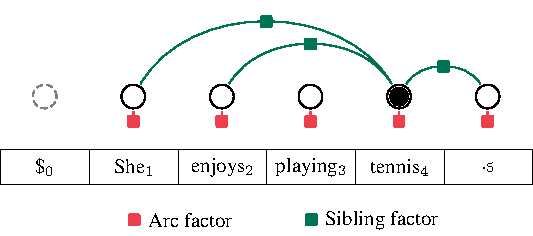
\includegraphics[scale=1]{figures/dep-factors.pdf}
        \caption{依存句法模型的因子图}
        \label{fig:con-factors}
    \end{subfigure}
    \begin{subfigure}[b]{0.8\textwidth}
        \centering
        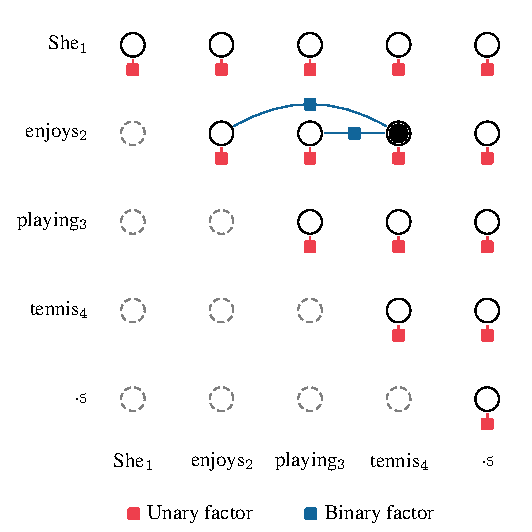
\includegraphics[scale=1]{figures/con-factors.pdf}
        \caption{成分句法模型的因子图}
        \label{fig:dep-factors}
    \end{subfigure}
    \caption{一个例句和其依存/成分句法模型对应的因子图,我们在例句上方标出了对应的正确无标签依存句法树和成分句法树,其中成分句法树进行了左二叉化.
        灰色虚线圆圈代表被屏蔽的变量.
        图中标出了所有的一阶(红色)因子,为了简洁起见,对于二阶因子,依存句法图中我们只标出了涉及弧$3\rightarrow 4$的兄弟(绿色)因子,成分句法图中只标出了和组块$(3, 4)$连接的二阶(蓝色)因子.}
    \label{fig:dep-vi-factors}
\end{figure}

\subsection{变分推断}

在得到分值之后,我们的句法分析方法分为两阶段:1)构建无标签树;2)预测标签.
在第二阶段预测标签的时候,我们以贪婪的方式给依存树的每条弧(见章节~\ref{sub@sec:dep-crf-labeling})或者成分树的每个组块(见章节~\ref{sub@sec:con-crf-model-definition})打上标签.
而在第一阶段构建无标签树时,我们的目的是选择后验概率最大的句法树$\hat{\boldsymbol{y}} = \arg\max_{\boldsymbol{y}} P(\boldsymbol{y}\mid \boldsymbol{x})$.
通常这样的推断的复杂度较高,以至于无法计算.
在句法分析领域我们可以应用Inside算法来进行精确计算,但是仍然十分影响计算效率.
因此在本节我们提出利用基于平均场理论的变分推断法来近似得到后验概率.
平均场变分推断假设句法树$\boldsymbol{y}$每个位置的变量相互独立,因此可以在线性时间内通过迭代的方法得到后验概率的近似值$Q(\boldsymbol{y})$.

关于平均场变分推断的通用更新公式以及相关推导见附录~\ref{appendix:mfvi-derivation}.
根据依存句法和成分句法任务目标的不同,我们在下面下面两小节详细阐述了通用公式针对具体任务的特化版本,以及相关的势函数(potential function)和因子图(factor graph)的设计.

\noindent\textbf{基于头选择的变分推断.}
依存句法模型的因子图见图~\ref{fig:dep-factors}

\noindent\textbf{基于二分类的变分推断.}
成分句法模型的因子图见图~\ref{fig:con-factors}

\subsection{训练}

\subsection{解码}

\subsection{复杂度分析}


\begin{figure}[tb]
    \centering
    \begin{subfigure}[b]{0.9\textwidth}
        \centering
        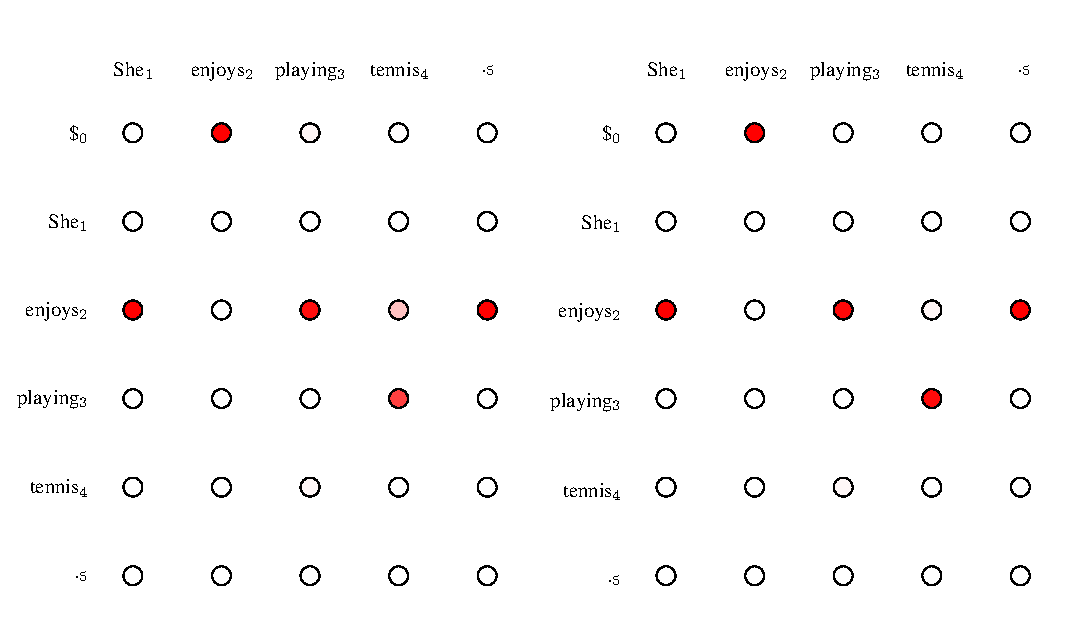
\includegraphics[scale=0.75]{figures/dep-probs.pdf}
        \caption{成分句法树每个位置对应的分值和后验概率}
        \label{fig:con-factors}
    \end{subfigure}
    \begin{subfigure}[b]{0.9\textwidth}
        \centering
        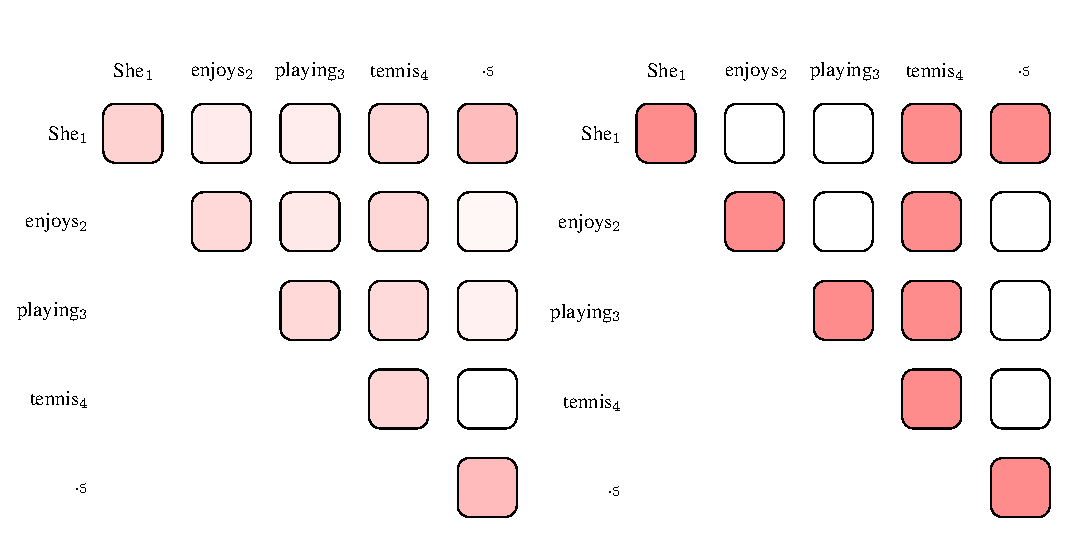
\includegraphics[scale=0.75]{figures/con-probs.pdf}
        \caption{成分句法树每个位置对应的分值和后验概率}
        \label{fig:dep-factors}
    \end{subfigure}
    \caption{一个例句对应的依存句法模型和成分句法模型的输出. 左边的图是每个位置的分值(log potential),为了方便显示,我们首先对分值进行了归一化.
        右边的图是变分推断得到的后验概率. 灰色虚线圆圈代表被屏蔽的不合法位置,颜色的深浅反应了分值/概率的大小.}

    \label{fig:dep-vi-factors}
\end{figure}

\section{实验}\label{sec:vi-exp}

\noindent\textbf{数据.}
为了方面和章节~\ref{cha:dep-crf}提出的精确推断的高阶模型进行比较,我们主要在英文的PTB和中文的CNLL09上进行了依存句法的实验.
同样的,我们在英文的PTB,中文的CTB51以及CTB7进行了成分句法分析实验.
实验数据的详细设置在章节~\ref{cha:dep-crf}和章节~\ref{cha:con-crf}有详细的设置,这里简洁起见不再重复.

\noindent\textbf{评价.}
在依存句法分析上,我们主要采用了有标签和无标签附着分值(UAS/LAS)作为评价指标,英文PTB的标点被忽略.
在成分句法分析上,我们采用了惯用的区块级别的准确率、召回率和F值(P/R/F)的指标,由标准工具\texttt{EVALB}来得到.
成分句法树在训练和评价时采用的预处理和后处理行为我们保持和章节~\ref{cha:con-crf}一致.

\noindent\textbf{参数设置.}
我们保持两种句法分析模型的编码器和训练方法与前面的章节基本一致.
对于二阶模型,我们设置依存句法分析中使用的兄弟特征以及成分句法分析使用的二阶特征的MLP层输出维度为100.
我们设置变分推断的迭代次数统一为3次.
在成分句法分析中我们新加入了一个参数$\lambda$来平衡标签和无标签树的训练损失,并设置$\lambda$为0.1.

\begin{table}[tb!]
  \centering
  \begin{tabular}{lcccc}
    \toprule
             & \multicolumn{2}{c}{PTB} & \multicolumn{2}{c}{CoNLL09}                 \\
             & UAS                     & LAS                         & UAS   & LAS   \\[2pt]
    \hline
    \\[-15pt]
    Baseline & 95.72                   & 93.97                       & 88.80 & 85.86 \\[3pt]
    LBP      &                         &                             &       &       \\
    MFVI     &                         &                             &       &       \\
    \bottomrule
  \end{tabular}
  \caption{Dev数据上的结果.}
  \label{table:dev-test}
\end{table}




\subsection{分析}

\noindent\textbf{子树和完全树的结果.}

\noindent\textbf{数据量的影响.}

\noindent\textbf{迭代次数的影响.}

\subsection{样例分析}

\subsection{速度比较}

\subsection{UD的结果}
